\documentclass[10pt, a4paper]{exam}
\usepackage{graphicx}
\usepackage[a4paper, total={7in, 9.5in}]{geometry}
\usepackage[normalem]{ulem}
\usepackage{amsmath}
\renewcommand\ULthickness{1.0pt}   
\setlength\ULdepth{1.3ex}

\begin{document}


	\noindent
	\begin{minipage}[l]{0.1\textwidth}
		\noindent
		
\includegraphics[width=2.8\textwidth]{ESCUDO.png}
	\end{minipage}
\hfill
\begin{minipage}[c]{0.8\textwidth}
	\begin{center}
		{\large  Departamento de Ingeniería civil y Agrícola\par
		\large	Facultad de Ingeniería	\par
	% \large \textbf{Taller propiedades de los fluidos}	\par
    \large \textbf{Banco de problemas\\Flujo variado - Estructuras Hidráulicas}	\par
} %%%%% NOMBRE DEL PROFESOR 
	\end{center}
\end{minipage}
\par
\vspace{0.2in}
\noindent
    \uline{Estructuras hidráulicas [2015954]	\hfill 2025-I}
\par 
\vspace{0.15in}
\noindent

%%%%%%%%%%%%%%%%%%%%%%%%%%%%%


En el presente taller se proponen un total de 25 ejercicios correspondientes a los temas \textit{Flujo variado y estructuras Hidráulicas}, se tiene así:

\begin{enumerate}


    \item  Water flows in a wide channel at $q = 10 \ \mathrm{m}^2/\mathrm{s}$ and $y_1 = 1.25 \ \mathrm{m}$. If the flow undergoes a hydraulic jump, calculate

        \begin{itemize}
            \item[(a)] $y_2$,
            \item[(b)] $v_2$,
            \item[(c)] $\mathrm{Fr}_2$,
            \item[(d)] $h_f$, and
            \item[(e)] the percentage dissipation of the energy.
        \end{itemize}


    \item Determine the upstream profile of a backwater curve given: $Q = 10 \ \mathrm{m}^3/\mathrm{s}$, \quad $b=3 \ \mathrm{m}$, \quad $\sin \theta = 0.001$, \quad $n = 0.022$.

    \begin{figure}[h]
        \centering
        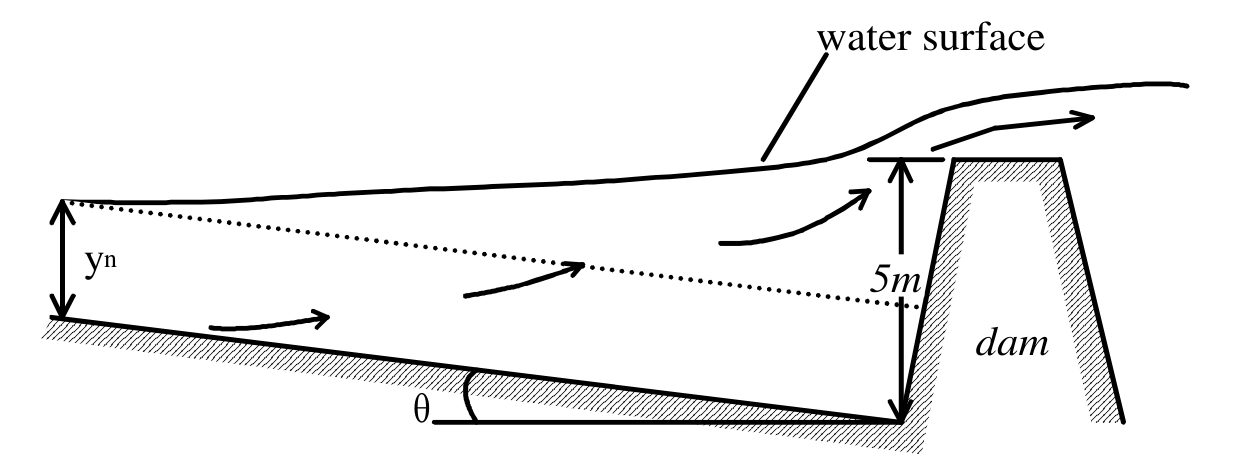
\includegraphics[width=0.44\linewidth]{Images/2.png}
        \caption{Perfil del problema.}
        \label{}
    \end{figure}

    \item  Sea un canal revestido de hormigón ($n = 0.011$) de sección trapecial simétrica de $7 \ \mathrm{m}$ de base e inclinación de los márgenes $1.5 \ \mathrm{H} : 1.0 \ \mathrm{V}$, cuya pendiente longitudinal es del $5\%$.

    Dicho canal une una balsa y una caída vertical que se encuentran separados $100 \ \mathrm{m}$ (véase la figura \ref{fig:3}). El nivel de la lámina de agua en la balsa se considera constante, siendo $1.54 \ \mathrm{m}$ la diferencia de cota entre la lámina de agua en la balsa y el lecho al inicio del canal. Determínese la profundidad en la sección de caída y el perfil de la lámina de agua con incrementos en la profundidad de $5 \ \mathrm{cm}$.

    \begin{figure}[h]
        \centering
        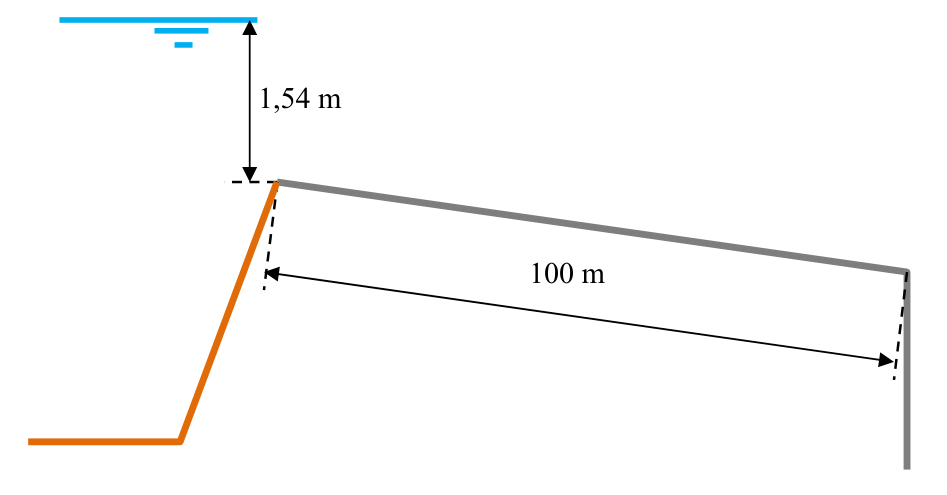
\includegraphics[width=0.5\linewidth]{Images/3.png}
        \caption{Condiciones y configuración iniciales del canal.}
        \label{fig:3}
    \end{figure}


    \item Sea un canal de longitud indefinida, sección rectangular con un $1\%$ de pendiente longitudinal, $3 \ \mathrm{m}$ de ancho y coeficiente de Manning de $0.018$, por el que circulan $4 \ \mathrm{m}^3 \cdot \mathrm{s}^{-1}$. Si en una determinada sección se encuentra una compuerta que permite el flujo únicamente a través de una abertura, limítrofe con el lecho, de $20 \ \mathrm{cm}$, determínese a qué distancia de la sección de la compuerta la profundidad de la corriente será de $40 \ \mathrm{cm}$.
    
    Especifíquese el tipo de perfil y dibújese con la curvatura (cóncava o convexa) adecuada.

    \item Sea un río de cauce prismático, longitud ilimitada y pendiente $1/10000$, cuya sección transversal tiene una anchura de $50 \ \mathrm{m}$ (supóngase $P \approx T$) y un coeficiente de Manning de $0.022$.
 
    Dicho río desemboca en un lago (véase la figura \ref{fig:5}). Determínese a qué distancia de la desembocadura el régimen del flujo puede considerarse aproximadamente uniforme, cuando circula un caudal de $63 \ \mathrm{m}^3 \cdot \mathrm{s}^{-1}$ y el nivel de agua en el lago es el que se muestra en la figura.

    Asimismo, dibújense y caracterísese los perfiles de flujo.

    \begin{figure}[h]
        \centering
        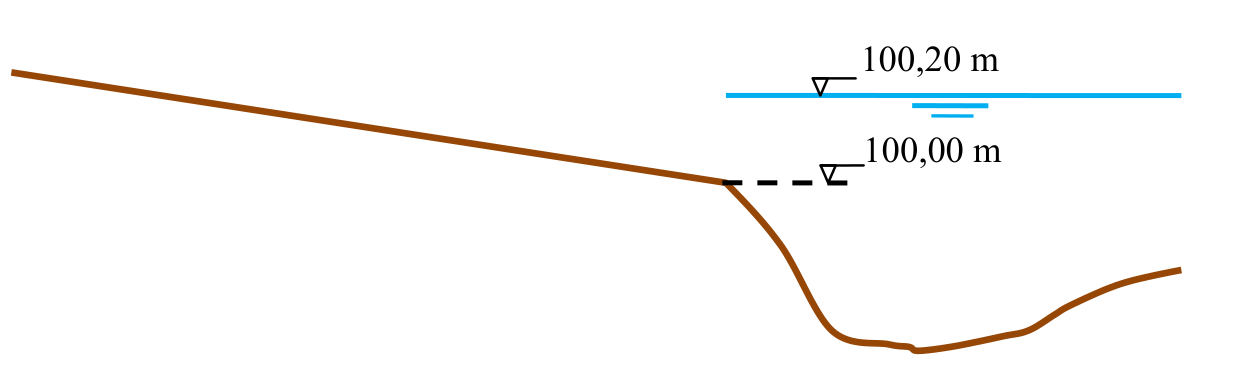
\includegraphics[width=0.5\linewidth]{Images/5.png}
        \caption{Condiciones y configuración iniciales del canal.}
        \label{fig:5}
    \end{figure}

    \item Sea un canal de mampostería con coeficiente de Manning igual a $0.028$, de sección rectangular de $9 \ \mathrm{m}$ de anchura, por el que circulan $30 \ \mathrm{m}^3 \cdot \mathrm{s}^{-1}$.

    Quedan diferenciados dos tramos en función de la pendiente longitudinal (véase la figura \ref{fig:6}). Uno, situado aguas arriba y de longitud indefinida, cuya pendiente es del $7\%$, y otro, aguas abajo, de $20 \ \mathrm{m}$ de longitud que finaliza en una caída vertical y cuya pendiente es del $2\%$.

    Dibújese de forma aproximada el perfil longitudinal de la lámina libre en los dos tramos, indicando el tipo de perfil y dibujándola con la curvatura (cóncava o convexa) adecuada.

    Asimismo, calcúlese a qué distancia de la caída vertical el calado será de $76 \ \mathrm{cm}$.

    \begin{figure}[h]
        \centering
        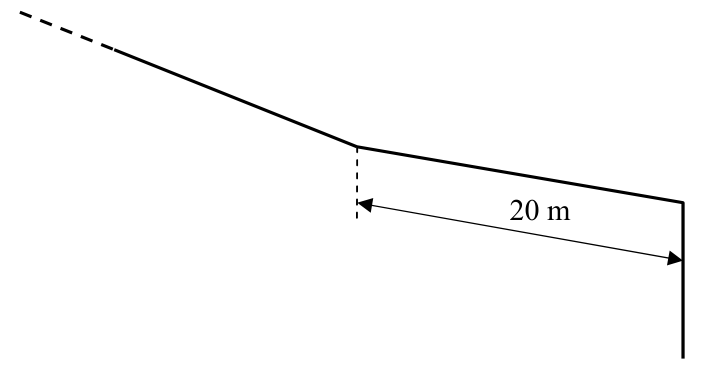
\includegraphics[width=0.5\linewidth]{Images/6.png}
        \caption{Condiciones y configuración iniciales del canal.}
        \label{fig:6}
    \end{figure}

    \item Sea un canal prismático de sección rectangular de $4 \ \mathrm{m}$ de ancho y coeficiente de Manning de $0.016$, por el que circulan $71 \ \mathrm{m}^3 \cdot \mathrm{s}^{-1}$.

    En función de la pendiente se distinguen dos tramos. Uno, aguas arriba, de longitud ilimitada y cuya profundidad normal es de $1.20 \ \mathrm{m}$. Otro, aguas abajo, construido en un Box-Culvert de $2 \ \mathrm{m}$ de altura, con pendiente del $1\%$, de $200 \ \mathrm{m}$ de longitud y que finaliza en una caída vertical (véase la figura \ref{fig:7}).

    Para las citadas condiciones:

    \begin{itemize}
        \item[(a)] Dibújese de forma aproximada el perfil longitudinal de la lámina libre del agua en los dos tramos, indicando el tipo de perfil.
        \item[(b)] Compruébese si el flujo circula en lámina libre a lo largo de todo el recorrido del Box-Culvert.
    \end{itemize}

\newpage

    \begin{figure}[h]
        \centering
        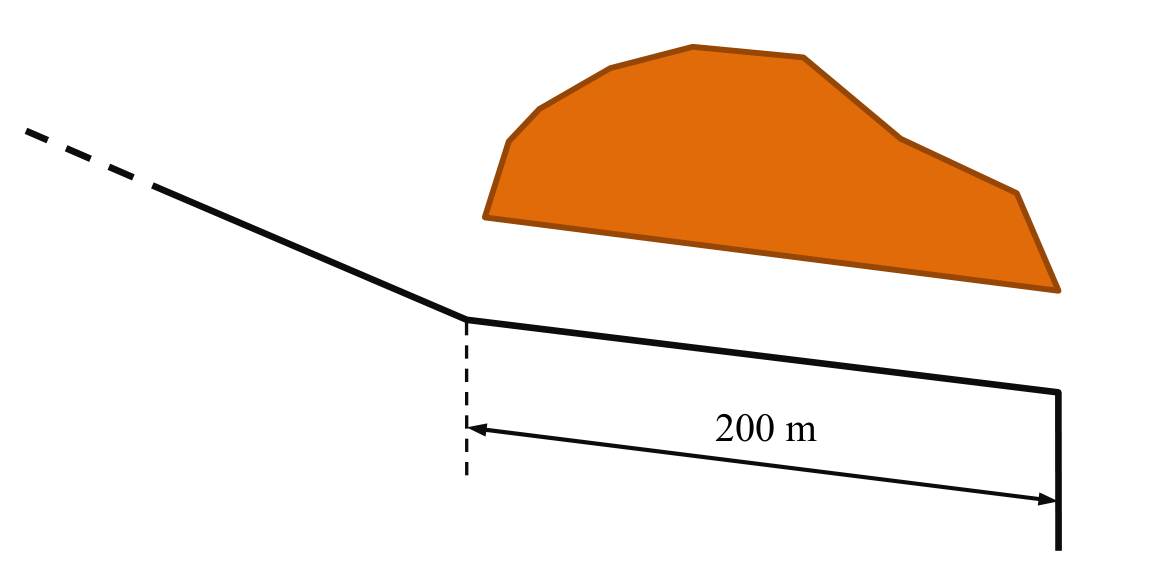
\includegraphics[width=0.5\linewidth]{Images/7.png}
        \caption{Condiciones del canal con Box-Culvert.}
        \label{fig:7}
    \end{figure}


    \item Sea un canal de mampostería ($n = 0.028$) de sección rectangular de $9 \ \mathrm{m}$ de anchura, por el que circulan $30 \ \mathrm{m}^3 \cdot \mathrm{s}^{-1}$.

    Se distinguen dos tramos en función de la pendiente longitudinal (que aumenta hacia aguas abajo). Uno, situado aguas arriba y de longitud indefinida, cuya pendiente es de $7 \ \mathrm{m}/\mathrm{km}$, y otro, aguas abajo, de $50 \ \mathrm{m}$ de longitud, que finaliza en una caída vertical y cuya pendiente es del $2\%$.

    En la sección en la que el canal cambia de pendiente se ubica una compuerta que únicamente permite el desagüe de fondo y cuya abertura para el presente caso es de $115 \ \mathrm{cm}$.

    Dibújese un esquema de la lámina de agua, especificando los perfiles que se dan en el canal, y calcúlese a qué distancia aguas arriba de la compuerta la profundidad será de $110 \ \mathrm{cm}$.

    \begin{figure}[h]
        \centering
        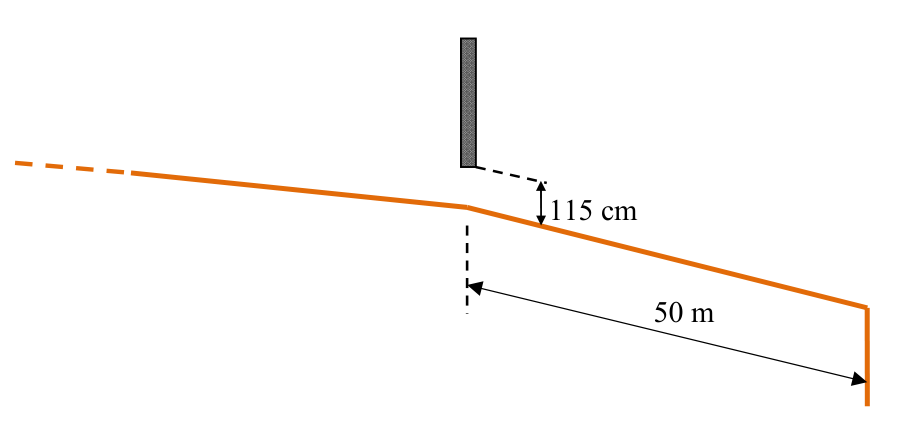
\includegraphics[width=0.5\linewidth]{Images/8.png}
        \caption{Condiciones del canal con compuerta.}
        \label{fig:8}
    \end{figure}

    \item Sea un cauce de sección rectangular de $14 \ \mathrm{m}$ de ancho y $n = 0.020$, por el que circulan $50 \ \mathrm{m}^3 \cdot \mathrm{s}^{-1}$.

    Se distinguen dos tramos en función de la pendiente longitudinal. Uno, situado aguas arriba y de longitud indefinida, cuya pendiente es $5 \cdot 10^{-4} \ (\mathrm{m} \cdot \mathrm{m}^{-1})$, y otro, aguas abajo, de $30 \ \mathrm{m}$ de longitud que finaliza en una caída vertical y cuya pendiente es del $1\%$.

    A $15 \ \mathrm{m}$ aguas arriba de la sección de caída se halla una compuerta con desagüe de fondo cuya abertura es de $90 \ \mathrm{cm}$ (véase la figura adjunta).

    Compruébese si en las condiciones descritas la compuerta influye en el flujo.

    \begin{figure}[h]
        \centering
        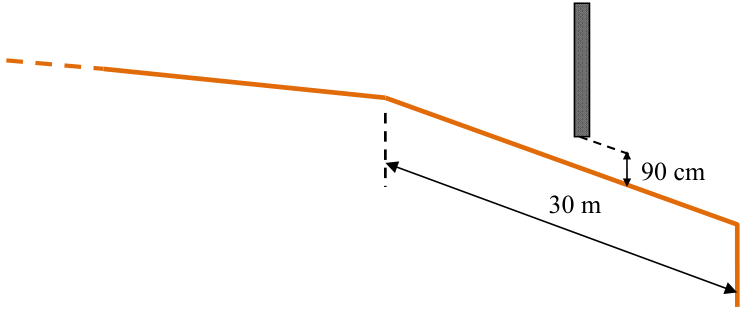
\includegraphics[width=0.47\linewidth]{Images/9.png}
        \caption{Condiciones del canal con compuerta.}
        \label{fig:9}
    \end{figure}


    \item  Considérese un cauce de sección rectangular de $15 \ \mathrm{m}$ de ancho y coeficiente de Manning de $0.030$, por el que circulan $12 \ \mathrm{m}^3 \cdot \mathrm{s}^{-1}$ en régimen permanente.

    Quedan diferenciados dos tramos en función de la pendiente longitudinal (véase la figura adjunta). Uno, situado aguas arriba y de longitud indefinida, cuya pendiente es $2 \cdot 10^{-3} \ (\mathrm{m} \cdot \mathrm{m}^{-1})$, y otro, aguas abajo, de $125 \ \mathrm{m}$ de longitud que desemboca en un lago de grandes dimensiones y cuya pendiente es del $2\%$.

    A $75 \ \mathrm{m}$ aguas arriba de la sección de cambio de pendiente se halla una estructura tipo compuerta a una altura de $2 \ \mathrm{m}$ sobre el lecho (véase la figura adjunta).

    Dibújese de forma aproximada el perfil longitudinal de la lámina libre en los dos tramos, indicando el tipo de perfil y dibujándola con la curvatura (cóncava o convexa) adecuada.

    Asimismo, compruébese si la estructura mencionada se encuentra separada del nivel de la superficie libre al menos $1.5 \ \mathrm{m}$ para el caudal circulante.

    \begin{figure}[h]
        \centering
        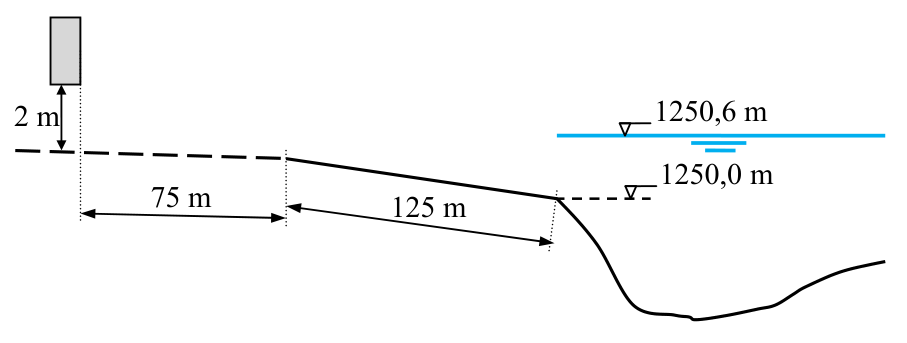
\includegraphics[width=0.47\linewidth]{Images/10.png}
        \caption{Condiciones del canal con compuerta.}
        \label{fig:10}
    \end{figure}

    \item En un canal rectangular de $1.5 \ \mathrm{m}$ de ancho se coloca un vertedero rectangular de pared delgada de $0.8 \ \mathrm{m}$ de longitud de cresta.

    Determine el caudal medio para una carga de $0.35 \ \mathrm{m}$.

    \begin{figure}[h]
        \centering
        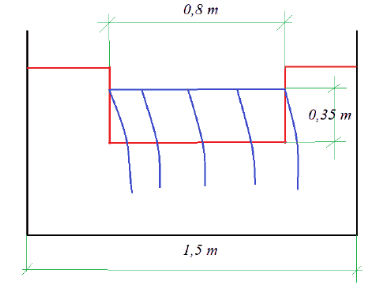
\includegraphics[width=0.35\linewidth]{Images/11.png}
        \caption{Vertedero de pared delgada.}
        \label{}
    \end{figure}

    \item A series of tests have been conducted to a vee weir of $90^\circ$. Determine the discharge coefficient ($C_d$) based on the following measured data.

    \begin{table}[h!]
    \centering
    \begin{tabular}{|c|c|c|c|c|c|c|c|c|}
    \hline
    $h_1$ (m) & 0.201 & 0.205 & 0.195 & 0.210 & 0.204 & 0.196 & 0.198 & 0.200 \\
    \hline
    $Q$ (L/s) & 25.1  & 25.4  & 25.0  & 25.6  & 25.5  & 24.9  & 24.9  & 25.1  \\
    \hline
    \end{tabular}
    \caption{Measured data for vee weir tests.}
    \label{}
\end{table}

    \item It is proposed to use a notch for measuring the water flow from a reservoir. It is estimated that the error in measuring the head above the bottom of the notch could be $1.5 \ \mathrm{mm}$. For a discharge of $0.3 \ \mathrm{m}^3/\mathrm{s}$, determine the percentage error which may occur, using a right-angled triangular notch with a coefficient of discharge of $0.6$.


    \item A rectangular channel $6 \ \mathrm{m}$ wide carries $168 \ \mathrm{lit}/\mathrm{min}$ at a depth of $0.9 \ \mathrm{m}$. What height of a rectangular weir must be installed to double the depth? Discharge coefficient of the weir may be taken as $0.85$.

    \item  A rectangular weir $0.75 \ \mathrm{m}$ high and $1.5 \ \mathrm{m}$ long is to be used for discharging water from a tank under a head of $0.5 \ \mathrm{m}$.

    Estimate the discharge:
    
    \begin{itemize}
        \item[(i)] When it is used as a suppressed weir
        \item[(ii)] When it is used as a contracted weir
    \end{itemize}

    Data: 
    
    \begin{itemize}
    \item Weir height ($P$) = $0.75 \ \mathrm{m}$
    \item Width of weir ($B$) = $1.5 \ \mathrm{m}$
    \item Head ($H$) = $0.5 \ \mathrm{m}$
    \end{itemize}
    
    Use Rehbock equation for estimating $C_d$ in both cases:
    
    \begin{equation}
        C_d = 0.605 + \frac{1}{1000H} + \frac{0.08 H}{P}
    \end{equation}
    
    \paragraph{Suppressed weir}
    
    \begin{equation}
        Q = C_d \, \frac{2}{3} \, B \, \sqrt{2g} \, H^{3/2}
    \end{equation}
    
    \paragraph{Contracted weir}
    \begin{equation}
        Q = C_d \, \frac{2}{3} \left( B - 0.1 \, n \, H \right) \sqrt{2g} \, H^{3/2}
    \end{equation}

    \item A weir of $8 \ \mathrm{m}$ long is to be built across a rectangular channel to discharge a flow of $9 \ \mathrm{m}^3/\mathrm{s}$.

    If the maximum depth of water on the upstream side of the weir is to be $2 \ \mathrm{m}$, what should be the height of the weir? Adopt $C_d = 0.62$. $L = 8 \ \mathrm{m}$, $Q = 9 \ \mathrm{m}^3/\mathrm{s}$, Depth of water = $2 \ \mathrm{m}$.


    \item Water is flowing over a trapezoidal weir of $4 \ \mathrm{m}$ long under a head of $1 \ \mathrm{m}$. Compute the discharge, if the coefficient of discharge for the weir is $0.62$.

    \item A narrow-crested weir of $10 \ \mathrm{m}$ long is discharging water under a constant head of $400 \ \mathrm{mm}$. Find the discharge over the weir in liters per second. Assume coefficient of discharge as $0.623$.

    \item Un vertedero Cipolletti de $0.80 \ \mathrm{m}$ de longitud de cresta y un vertedero triangular de $90^\circ$ deberán instalarse en la pared de un reservorio.

    Se desea saber qué distancia vertical deberá haber entre la cresta del Cipolletti y el vértice del triangular hasta que el gasto en ambos sea el mismo e igual a $800 \ \mathrm{l/s}$.

    ¿Cuál es la carga sobre cada uno de los vertederos?

    \subsection*{Datos}
    
    \begin{table}[h!]
    \centering
    \begin{tabular}{|c|c|c|c|}
    \hline
    \textbf{Cipolletti} & b = $0.8$ & Q = $800 \ \mathrm{l/s}$ &  \\ 
    \hline
    \textbf{Triangular} & $\theta = 90^\circ$ & C = $0.60$ & Q = $800 \ \mathrm{l/s}$ \\
    \hline
    \end{tabular}
    \caption{Datos para los vertederos Cipolletti y triangular.}
    \label{tab:vertedero_datos}
    \end{table}

    \begin{figure}[h]
        \centering
        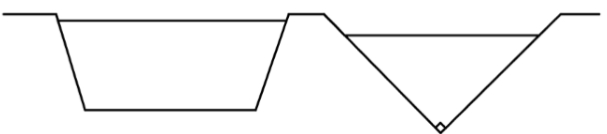
\includegraphics[width=0.4\linewidth]{Images/19.png}
        \caption{Configuraciones de los vertederos.}
        \label{}
    \end{figure}

\newpage

    \item  Determinar la velocidad de flujo sobre el vertedero de ranura en V a $60^\circ$, si el ancho de ranura en la parte superior es de $12''$ ($C_d = 0.60$).
    
    \begin{figure}[h]
        \centering
        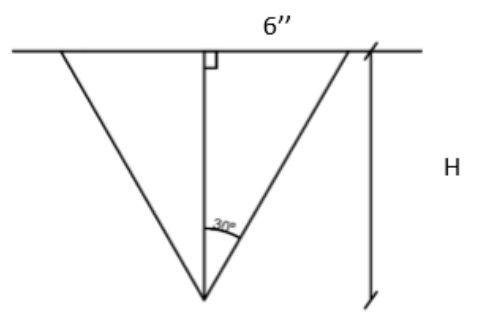
\includegraphics[width=0.35\linewidth]{Images/20.png}
        \caption{Configuración del vertedero triangular.}
        \label{}
    \end{figure}
    
    \item Sobre una placa con las dimensiones que se presentan en la figura 7.5 se produce un vertido superior y una descarga por el orificio del fondo. El ancho de la placa es de $1.00 \ \mathrm{m}$ y es igual al del canal.

    Determinar cuál es el gasto de vertido si el del orificio es $Q_o = 0.3 \ \mathrm{m}^3/\mathrm{s}$, suponiendo que en ambos la descarga es libre. Asuma un $C_d=0.595$  

    \begin{figure}[h]
        \centering
        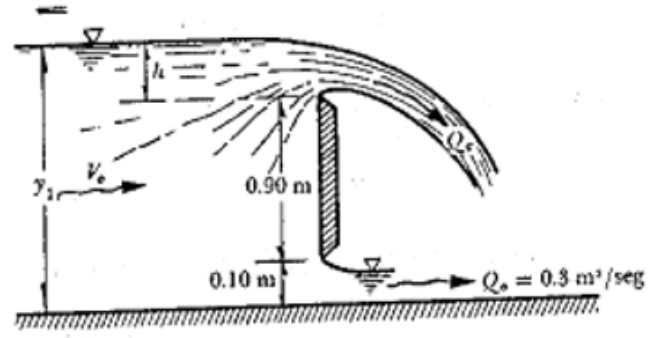
\includegraphics[width=0.4\linewidth]{Images/21.png}
        \caption{Configuración del vertedero y el orificio.}
        \label{}
    \end{figure}


    \item Water flows down a channel at a rate of $0.053 \ \mathrm{m}^3/\mathrm{s}$. What would be the head over a rectangular weir and triangular (v-notch) weir at this discharge if the rectangular weir has a crest length of $0.3 \ \mathrm{m}$ and the triangular weir has a total angle of $60^\circ$? Ignore the velocity of approach and the effect of side contractions when dealing with the rectangular weir and take $C_d$ for both weirs as $0.60$.


    \item El orificio circular practicado en la pared vertical de un recipiente que contiene agua, tiene un diámetro $D = 0.10 \ \mathrm{m}$ y desaloja un caudal $Q = 29.5 \ \mathrm{l/s}$ con una altura de carga $H = 2 \ \mathrm{m}$.
    
    Con el sistema de coordenadas indicado en la figura, se ha medido en el laboratorio que $x = 3 \ \mathrm{m}$ y $y = 1.15 \ \mathrm{m}$, para el punto 1.
    
    Calcular los coeficientes de contracción, Caudal (coeficiente de descarga) y velocidad.

    \begin{figure}[h]
        \centering
        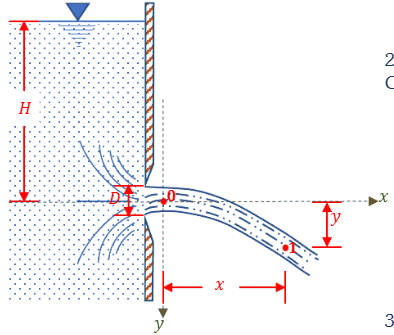
\includegraphics[width=0.29\linewidth]{Images/23.png}
        \caption{Configuración del orificio.}
        \label{}
    \end{figure}
    
    \item Por un canal rectangular de ancho $2.0 \ \mathrm{m}$ circula agua con caudales entre $Q_\mathrm{min} = 20 \ \mathrm{l/s}$ y $Q_\mathrm{max} = 600 \ \mathrm{l/s}$.
    
    Este caudal se debe medir usando:
    
    \begin{itemize}
        \item Un vertedero rectangular de pared delgada (sin contracción)
        \item Un vertedero triangular de pared delgada con una abertura de $90^\circ$
        \item Un vertedero de pared gruesa
    \end{itemize}
    
    En todos los casos $P = 1.0 \ \mathrm{m}$. Hacer una gráfica de $H$ (vertical) vs $Q$ (horizontal) para cada vertedero e indique cuál vertedero sería el mejor para esta aplicación.



    \item Se ha instalado un vertedero rectangular ($C_d = 0.6$) de $1 \ \mathrm{m}$ de ancho en el extremo de aguas abajo de un canal rectangular del mismo ancho.

    Determinar la fuerza horizontal que debe suministrar la cimentación para evitar que el vertedero sea arrastrado por la corriente. ($\alpha = \beta = 1$).

    \begin{figure}[h]
        \centering
        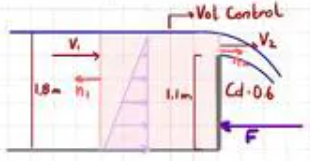
\includegraphics[width=0.4\linewidth]{Images/25.png}
        \caption{Configuración del problema.}
        \label{}
    \end{figure}



\end{enumerate}

    
\end{document}



